\documentclass[11pt]{article}
\usepackage{fullpage}
\usepackage{graphicx}

\title{Project Plan}
\date{}

\setlength{\parskip}{\baselineskip}%
\setlength{\parindent}{0pt}%

\begin{document}
\maketitle
\tableofcontents
\newpage
\section{Introduction}

The primary aim for this software project is to develop a competitive strategy game to between two or more players.

Each of the players design an \textit{ant brain}, which is a file containing instructions for ants to carry out in a simulated ant world. The ant brains will contain instructions on how the ants will react based on their current state and the local environment. Once loaded into the program, two colonies of ants compete in a simulated ant-world to bring as much food as possible back to their anthill. The ant world contains obstacles, food, and the two opposing anthills. Ants are able to leave markers for other ants to sense, and can also kill opponent ants by surrounding them. The game is won by the ant colony which obtains the most food.

As specified by the client, the produced software must have the ability to:
\begin{itemize}
\item check if an ant-brain supplied by a player is syntactically well-formed.
\item check if a given description of an ant world is syntactically well-formed and meets the requirements for ant worlds used in tournaments.
\item visualise a given ant world.
\item generate random but well-formed ant worlds.
\item simulate an ant-world: that is, enable two players to upload their ant-brains and choose an ant-world, and then run the game in the ant world, taking statistics and determining the winner of the game.
\item play tournaments, where an arbitrary number of players can upload ant-brains, who are all paired up to play against each other.
\end{itemize}

In addition, a custom ant-brain should be designed.

\newpage
\section{Phase Plan}

\subsection{Phase Summary}

The first week of the project shall involve preparation of organisational documents and team organisation. In addition, development environments and general project configuration shall be set up - this includes version control and communication channels. The preparation phase should be complete by 28/02/2016 at the latest.

In the next week, the project plan shall be developed by the team. The primary components of the project plan shall include a protocol for conflict resolution, a full and detailed phase plan (including PERT chart), and an assessment plan. Alongside the plan, he team shall work in parallel to identify the functional, non-functional and domain requirements. Where any domain requirements are discovered, they shall be filtered into functional/non-functional requirements after discussion with the group. This phase shall be completed by 07/03/2016 at the latest.

Once the requirements are complete, the design phase will begin. This is the longest (and most challenging) phase, and shall be split up amongst the team based on the categories of functional (and non-functional) requirements. The first stage of the design phase shall be to identify key components of the software and identify the associations between them, forming a high-level design. Next, a lower level design shall be developed through the use of class diagrams (UML) and sequence diagrams. The design should be complete by 29/03/2016.

Next is the development phase. Again, the team will split into groups to work in parallel - with some members mainly focused on development and others focused on writing tests. The development shall follow the design specification as closely as possible, and where any ambiguities arise both the requirements and design will be revised where necessary. The development should be complete by 23/04/2016.

After development is complete, there shall be a final validation and completion phase. This will involve performing checks on the software (unit testing, verification, validation, release testing). In addition, user documentation for the program will be finalised, a custom ant-brain shall be designed, and a team report shall be written. These final tasks must be completed before the project deadline, 05/05/2016.

\subsection{Task Allocation and Time Estimation}

The following table gives an approximate optimistic-realistic-pessimistic estimation for the time spent on each task in the project. All times are given in days.

\begin{center}
\begin{tabular}{|l|l|l|l|l|}
\hline
\textbf{Task} & \textbf{Optimistic} & \textbf{Realistic} & \textbf{Pessimistic} & \textbf{Allocated}  \\ \hline
\multicolumn{5}{|l|}{\textbf{Preparation}} \\ \hline
Team Organisation & 1 & 2 & 3 & Sal \\ \hline
Configuration Management & 2 & 3 & 5 & Sam \\ \hline
\multicolumn{5}{|l|}{\textbf{Plan}} \\ \hline
Conflict Resolution & 1 & 2 & 3 & Dan \\ \hline
Phase Plan & 4 & 7 & 10 & Jeremiah \\ \hline
Organisation Plan & 3 & 5 & 7 & Sal\\ \hline
Peer Assessment Plan & 1 & 2 & 3 & Dan \\ \hline
\multicolumn{5}{|l|}{\textbf{Protocols}} \\ \hline
Acceptance Criteria & 2 & 3 & 4 & Dan \\ \hline
Development Protocols & 1 & 2 & 3 & Sam \\ \hline
Test Specification & 4 & 5 & 7 & Sam, Sal \\ \hline
\multicolumn{5}{|l|}{\textbf{Requirements}} \\ \hline
Functional & 5 & 8 & 11 & Kea, Regan \\ \hline
Non-Functional & 3 & 6 & 9 & Sam \\ \hline
Domain & 1 & 2 & 3 & Sam \\ \hline
\multicolumn{5}{|l|}{\textbf{Design}} \\ \hline
High $\rightarrow$ Low-Level & 20 & 22 & 24 & All \\ \hline
\multicolumn{5}{|l|}{\textbf{Development}} \\ \hline
Programming & 20 & 25 & 30 & Regan, Sam \\ \hline
Documentation & 5 & 7 & 9 & Dan \\ \hline
Unit Testing & 10 & 12 & 14 & Sal, Jeremiah \\ \hline
\multicolumn{5}{|l|}{\textbf{Validation}} \\ \hline
Component Testing & 7 & 9 & 11 & Sal, Jeremiah \\ \hline
\multicolumn{5}{|l|}{\textbf{Other}} \\ \hline
User Documentation & 7 & 9 & 11 & Dan \\ \hline
Report & 2 & 3 & 4 & All \\ \hline
Custom Ant Brain & 2 & 4 & 6 & Jeremiah \\ \hline
\end{tabular}
\end{center}

\subsection{PERT Chart}

The PERT chart below shows the main phases of the project. It is assumed that the subtasks of each phase (as in the task times table) can be worked on asynchronously by the team, so the longest sub-task for each phase has been used to characterise the total completion time of each phase. In the chart the \texttt{(x, y, z)} tuple below each node is the optimistic, realistic and pessimistic completion time in days. The realistic completion time has been used to calculate the critical path (the path marked with red arrows).

\begin{center}
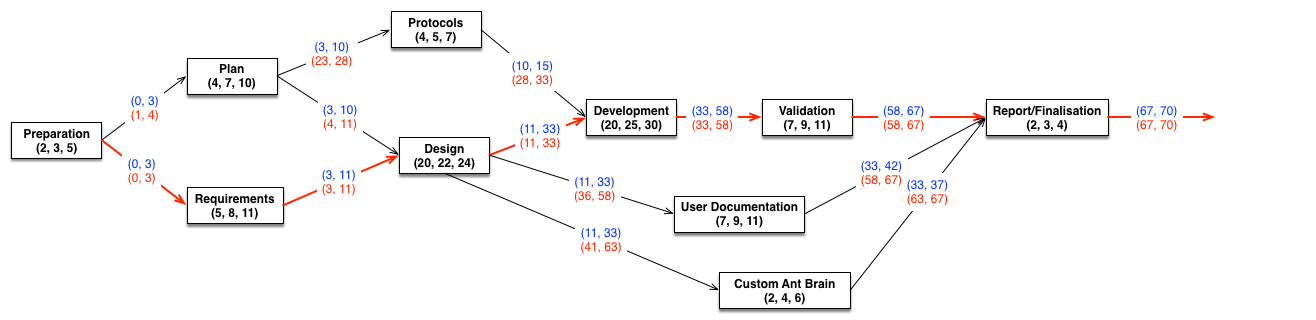
\includegraphics[width=\linewidth]{resources/pert}
\end{center}


The project was started by the group on 18/02/2016. This means, assuming each phase on the critical path is completed in exactly the above 'realistic' number of days, the completion date of the project should be 28/04/2016. This gives 8 days of freedom in the critical path before the project deadline.

\subsection{Deadlines}

From the above PERT chart, to finish the project on time the strict completion deadlines are:

\begin{center}
\begin{tabular}{|l|l|}
\hline
\textbf{Task} & \textbf{Date} \\ \hline
Preparation Complete & 28/02/2016 \\ \hline
Plan Complete & 07/03/2016 \\ \hline
Requirements Complete & 07/03/2016 \\ \hline
Design Complete & 29/03/2016 \\ \hline
Protocols Complete & 29/03/2016 \\ \hline
Development Complete & 23/04/2016 \\ \hline
Validation Complete & 02/05/2016 \\ \hline
User Documentation Complete & 02/05/2016 \\ \hline
Report/Finalisation Complete & 05/05/2016 \\ \hline
\end{tabular}
\end{center}

\subsection{Phase Descriptions}

\subsubsection{Planning and Documentation}

This phase of the project will involve the writing up and compilation of multiple different documents, plans and reviews that will detail relevant information and specifications relating to the project team, the client, and the project itself. It is also fair to assume some documentation may need to be completed or be updated over the course of the project. However, the majority should be produced at this stage. The main documents to be produced at this stage should include the following:
\begin{itemize}
\item Organisation plan
\item Phase plan
\item Requirements specification (functional, non-functional and domain)
\item Risk assessment
\item Conflict resolution plan
\item Project plan
\item Peer assessment plan
\item PERT chart
\end{itemize}
Further documentation includes the user documentation and acceptance criteria, which are provided in separate documents.

\subsubsection{Design}

The design phase of the project will involve drawing up, analysing and deciding upon the design of the ant game within the confines of the requirements (given in the requirements document). As a result, this part of the project will lead to useful documents, specifically containing UML and sequence diagrams. The documents to be produced are first a high-level design specification, and then a detailed design specification

The design phase will be very important for trying to implement a successful ant game and, in particular, understanding the fundamentals of how our team will go about making the game and the different aspects of it (e.g. ant brain, world viewer, GUI).

\subsubsection{Implementation}

This phase of the project will involve writing up the code for and implementation of the ant game, based on the specifications given from the design phase and the requirements document. The elements to be coded for and implemented are specified in the requirements document.

This stage in the project will have the members of the team working, both in some parts individually and in other parts together, on programming the code for the mentioned elements. Simpler elements to be coded for can be done individually, whereas harder components to code for will be worked on in pairs/subgroups.

\subsubsection{Testing}

The testing phase of the project will for the most part run simultaneously alongside coding. This will make the coding process run more smoothly and identify problems and errors early, which should aid to prevent potentially more difficult complications (allowing time to be saved that would otherwise be spent looking for errors) further down the line. This phase will have to be run according to a test specification that will highlight how the tests should work.

\newpage
\section{Risk Management}
\subsection{Risk Identification and Analysis}

\begin{center}
\begin{tabular}{|p{0.4\textwidth}|l|l|l|l|}
\hline
\textbf{Risk} & \textbf{Key} & \textbf{Probability} & \textbf{Effect} & \textbf{Type} \\ \hline
Documents become lost/corrupt due to various circumstances. & 1 & Moderate & Serious & Technology \\ \hline
A member leaves the team before project completion. & 2 & Low & Serious & Organisational \\ \hline
Members are unable to meet a deadline. & 3 & Moderate & Serious & People \\ \hline
The customer changes the requirements mid-process. & 4 & High & Serious & Requirements \\ \hline
A piece of software is buggy, unable to work accordingly. & 5 & Moderate & Serious & Tools \\ \hline
There is conflict in the team that requires management of some sort. & 6 & Moderate & Serious & People \\ \hline
The time to complete an objective was underestimated. & 7 & Moderate & Serious & Estimation \\ \hline
The size/difficulty of a task was underestimated. & 8 & High & Tolerable & Estimation \\ \hline
The tests needed to adequately check the code was under-developed. & 9 & Moderate & Tolerable & Estimation \\ \hline
Code generated is inadequate for the particular objective. & 10 & Moderate & Tolerable & Requirements \\ \hline
Organisation of team is restructured, meaning someone else is in control. & 11 & Low & Tolerable & Organisational \\ \hline
Member late due to uncontrollable circumstances. & 12 & High & Insignificant & People \\ \hline
Members absent for meeting. & 13 & Moderate & Insignificant & People \\ \hline
\end{tabular}
\end{center}

\subsection{Risk Indicators}

\begin{center}
\begin{tabular}{|l|p{0.8\textwidth}|}
\hline
\textbf{Risk Type} & \textbf{Description} \\ \hline
Technology & There are many cases of technology problems. Any task undertaken on a certain software takes longer than predicted. \\ \hline
People & Poor staff morale. Poor relationships amongst team members. High levels of lateness/absence. \\ \hline
Organisational & Lack of action by members. Lack of work being done. \\ \hline
Tools & Reluctance by team members to use tools or requests for other types of tool. \\ \hline
Requirements & There are many requests for the change in requirements, or customer complaints. \\ \hline
Estimation & Failure to meet agreed schedule. Failure to clear reported defects. \\ \hline
\end{tabular}
\end{center}

\subsection{Risk Planning}

\begin{enumerate}
\item For a file/piece of code, as soon as a sizeable update is made to it, can be backed up via an external memory device, as well as uploaded to sharing software, i.e. GitHub.
\item As all members are involved in various degrees in all areas, a void in one area can be filled by a combination of the others.
\item The democratic decentralised nature of the organization allows members to switch to other areas if someone is unable to undertake their task on time. 
\item Derive traceability information to assess how the change impacts the project, impact; as well as maximize information hiding in the design to limit the effect of any change. 
\item Make a list of several systems/software per usage, so if one fails then there are others known that can replace it. 
\item \begin{enumerate}
  \item Arrange a team meeting to settle any disputes, more civilised general request.
  \item Senior/other member speak to each involved individual separately to gather information to make a decision, or to manage them separately.
  \item Forcefully request members to solve dispute.
  \item Ask for outside aid, either from `client' or higher management to put the conflicting members back into place. 
\end{enumerate}
\item If code is taking longer, prioritise certain aspects, to focus on the vital elements, with parts i.e. the GUI created in simpler formats. If a certain piece of documentation is obstructing the start/continuation of the coding, perhaps leave it till later if not vital to the design/later implementation or testing phases. Once more, the organisation of the team allows small shifts in focus if necessary. 
\item Same as 7.
\item If time isn’t at a premium, focus more on the testing, as that can show how well the code runs the game, and how much, if any tinkering with the code is needed. 
\item Either via testing, or by looking back at the designs, focus on improving code incrementally, slowly building it up to what it should be. Look at code comments to see if something is missing that prevents full operation of that class/method etc. 
\item The team layout means there is little affect, as people know at least the basic of each area of the project, requiring only a little update, perhaps by looking back at previous documentation, to get a full scope of the area. 
\item The minutes of the meetings are recorded, so little vital information is ever missed.
\item The contents of a meeting are noted, and then uploaded, allowing for absentees to catch up.
\end{enumerate}

\newpage
\section{Organisation Plan}

\subsection{Configuration Management}

\subsubsection{Communication and Version Control}

The main communication channel will be Slack where discussions will take place, whereas for information sharing of technical documents Github will be used as it includes version control procedures making it easier to make changes. There is a strict requirement for each member to record documents they upload and edit, consisting of the document name, author, auditor, version number and last modification date. This requirement will be satisfied by using the Git version control system. When a document is uploaded or edited, it is automatically communicated across in Slack. Edited and uploaded documents shall be reviewed at the next meeting before being marked as completed by the team as further changes may be required. If changes are required this shall be communicated in Slack or in a team meeting and will be later implemented. Team communication relevant to the product-related aspects of the project (planning, development, testing) shall be recorded for future reference:
\begin{enumerate}
\item Facebook chat - message archive
\item Slack chat - message archive
\item In-person - meeting minutes
\end{enumerate}

\subsubsection{Development}

The below is relevant configuration information which has been extracted from the non-functional requirements document.

\begin{itemize}
\item All development and testing shall be undertaken in either the Netbeans IDE, Eclipse IDE, or IntelliJ IDE.
\item JUnit 4.12 shall be used as the testing library across all development and testing systems.
\item Gradle 2.5+ shall be used as the build automaton system across all development and testing systems.
\item All project-related documents, source code, tests and builds shall be kept on the team’s GitHub repository, with new versions being committed and pushed to the repository on a regular basis and as soon as a major change/refactoring occurs.
\item A copy of all project documents and source code shall be stored independently on each team member’s personal computer, regularly pulled from the central team GitHub repository. In addition, an up-to-date backup of the GitHub repository shall be kept in one or more of the team’s personal Dropbox repositories.
\item The Jacoco code coverage analysis tool shall be used by the testing/validation team to ensure maximum code coverage.
\end{itemize}

Note: The Jacoco and JUnit tools are automatically set up using Gradle and the gradle build file, which is stored
on the central repository.

\subsection{Roles}

\subsubsection{Allocation}

The team consists of Sam, Kea, Jeremiah, Regan and Arsalan. The project manager and technical leader will be Sam, who will be responsible for critical technical decisions. However the team structure is primarily \textit{decentralised democratic} and therefore decisions are primarily formulated as a team. Kea, Dan and Jeremiah will take part in analysis, who will formulate ideas with the design team composed of Arsalan and Dan. Arsalan and Dan will communicate with the programming team composed of Regan and Sam to discuss feasible design aspects. Finally, Jeremiah and Arsalan will be part of quality assurance working with Regan and Sam to discuss solutions to potential or exposed problems. The PERT chart and the management of documentation will be managed by Kea, Jeremiah and Sam who will work with the rest of the team to ensure the project is on track.

\subsubsection{Analysis}

The overall responsibilities of the analysis team will be to read the project brief in detail and work on the requirements engineering document. This requirements document will denote all required functionality of the system and its constraints. The next step will be to communicate this across to the design team, who will read the specification and use it as an aid to the design process. The final step is to make any required changes/clarifications to the design team if a requirement is not fully understood.

\subsubsection{Design}

The overall responsibilities of the design group will be to meet the software specification outlined by the analysis team. The team will establish an overall architecture for the system by implementing a high level and detailed design by providing appropriate design documentation in UML. In addition, detailed sequence diagrams will be developed. The produced documents will represent the abstractions identified by the analysis team and will formulate these into relationships, which will later be used by the programming team as aids to the implementation of the project. The next step is to refactor the design for the case of the programming team identifying design flaws.

\subsubsection{Programming}

The overall responsibilities of the programming team will be to implement the design effectively using the supplied documentation, whilst also communicating with the design team any potential flaws in the design. The programming team will also work with quality assurance by helping to supply an effective test plan. The programming team will also have an ongoing of step of refactoring any code for the case of design changes communicated by the design team.

\subsubsection{Quality Assurance}

Quality Assurance will ensure the programming team's implemented solution is thoroughly tested against the requirements identified by the analysis team. They will communicate any errors which fail to meet these requirements up to the programming team, who will make the required changes if necessary. QA will first implement a test plan whilst working with the programming team and design team. They will then will physically carry out various forms of testing.

\newpage
\section{Peer Assessment Plan}

Being a group project, the first aim is to produce the best ant game possible, but each individual will be reviewed in order to devise some sort of grading system to reward all those who perform well. The three primary areas are work, attendance and social behaviour. 

The primary target for which each member shall be judged is that they take an active role in the work. Everyone must do a fair amount of work, and that work must be submitted to the team at the given deadlines. Failure to do so will mean a lower end grade. Of course, the quality of work must be to a decent standard, since there is little use only doing the basic work with little care or thought. 

Members' overall attendance must also be considered --- attendance of meetings, both in the seminars and out-of-class. This demonstrates the individuals level of commitment to both the project and in particular the team, as it proves they are ready to help the other members. They must then, during said meetings, take part and have discussions with the group, in order to help both themselves and others understand what is being asked. 

The final area that members will be assessed on is the social side of the group. They should be active during social discussions across the media/ other forms of communication. This makes sure that all members are `kept in the loop', and at all times they are fully aware of the situation. It must be noted that any limitations such as lack of internet access will be considered and accounted for when the final assessment is given. All members, if needed, should try and dissolve any arguing within the group, which will of course make the project run smoothly and keep up moral. The final point in this area is a simple `treat others like you would yourself' approach, where all members are expected to be kind and generous to each other to make sure that everyone has an equal voice, per the choice of group structure. 

By each member performing well in each of the three areas, the project will be completed on time and to a high standard. This makes it imperative that each member, whilst thinking of how well they are performing in relation to their end mark, always has the team and the project at the forefront of their minds. 

The end scores in each area, and thus the overall mark, will be discussed and calculated at the end of the project when everything else is completed. By looking back over the team meeting minutes, as well as the activity sheets, the performance of each member will be seen. These both will show how well each member did in the attendance and work areas, with the social area being fairly evaluated as a group. If a member does not agree with their marking it can be discussed as a group, allowing an overall opinion to be reached --- further disagreement can be taken up with the ‘client’. 

Finally, each member must be in full agreement with the final peer assessment. When this final deliverable is submitted, each member must sign off on it, ensuring full agreement and compliance with what is to be contained.  

\end{document}
